\documentclass[11pt, onecolumn]{report}
\newcommand{\Define}{\stackrel{\triangle}{=}}
\newcommand{\argmin}{\operatornamewithlimits{argmin}}
\newcommand{\argmax}{\operatornamewithlimits{argmax}}
\usepackage{underlin}
\usepackage{algorithmic}
\usepackage{algorithm}
\usepackage{multirow}
\usepackage{subfigure}
\usepackage{cite}
\usepackage{latexsym}
\usepackage{verbatim}
\usepackage{amssymb}
\newtheorem{thm}{\bf Theorem}
\newtheorem{cor}[thm]{Corollary}
\newtheorem{lem}{{ Lemma}}
\usepackage{graphicx}
\usepackage{epsf}
\usepackage{color}
\usepackage{epsfig}
\usepackage[cmex10]{amsmath}
\usepackage{graphicx,wrapfig,lipsum}
\usepackage{glossary}
\usepackage{textcomp}
%\usepackage{hyperref}
\usepackage{amsmath}
\usepackage{arydshln}
% Psfig/TeX 
\def\PsfigVersion{1.10}
\def\setDriver{\DvipsDriver} % \DvipsDriver or \OzTeXDriver
%
% All software, documentation, and related files in this distribution of
% psfig/tex are Copyright 1993 Trevor J. Darrell
%
% Permission is granted for use and non-profit distribution of psfig/tex 
% providing that this notice is clearly maintained. The right to
% distribute any portion of psfig/tex for profit or as part of any commercial
% product is specifically reserved for the author(s) of that portion.
%
% To use with LaTeX, use \documentstyle[psfig,...]{...}
% To use with TeX, use \input psfig.sty
%
% Bugs and improvements to trevor@media.mit.edu.
%
% Thanks to Ned Batchelder, Greg Hager (GDH), J. Daniel Smith (JDS),
% Tom Rokicki (TR), Robert Russell (RR), George V. Reilly (GVR),
% Ken McGlothlen (KHC), Baron Grey (BG), Gerhard Tobermann (GT).
% and all others who have contributed code and comments to this project!
%
% ======================================================================
% Modification History:
%
%  9 Oct 1990   JDS	used more robust bbox reading code from Tom Rokicki
% 29 Mar 1991   JDS	implemented rotation= option
% 25 Jun 1991   RR	if bb specified on cmd line don't check
%			for .ps file.
%  3 Jul 1991	JDS	check if file already read in once
%  4 Sep 1991	JDS	fixed incorrect computation of rotated
%			bounding box
% 25 Sep 1991	GVR	expanded synopsis of \psfig
% 14 Oct 1991	JDS	\fbox code from LaTeX so \psdraft works with TeX
%			changed \typeout to \ps@typeout
% 17 Oct 1991	JDS	added \psscalefirst and \psrotatefirst
% 23 Jun 1993   KHC     ``doclip'' must appear before ``rotate''
% 27 Oct 1993   TJD	removed printing of filename to avoid 
%			underscore problems. changed \frame to \fbox.
%			Added OzTeX support from BG. Added new
%			figure search path code from GT.
%
% ======================================================================
%
% Command synopsis:
%
% \psdraft	draws an outline box, but doesn't include the figure
%		in the DVI file.  Useful for previewing.
%
% \psfull	includes the figure in the DVI file (default).
%
% \psscalefirst width= or height= specifies the size of the figure
% 		before rotation.
% \psrotatefirst (default) width= or height= specifies the size of the
% 		 figure after rotation.  Asymetric figures will
% 		 appear to shrink.
%
% \psfigurepath{dir:dir:...}  sets the path to search for the figure
%
% \psfig
% usage: \psfig{file=, figure=, height=, width=,
%			bbllx=, bblly=, bburx=, bbury=,
%			rheight=, rwidth=, clip=, angle=, silent=}
%
%	"file" is the filename.  If no path name is specified and the
%		file is not found in the current directory,
%		it will be looked for in directory \psfigurepath.
%	"figure" is a synonym for "file".
%	By default, the width and height of the figure are taken from
%		the BoundingBox of the figure.
%	If "width" is specified, the figure is scaled so that it has
%		the specified width.  Its height changes proportionately.
%	If "height" is specified, the figure is scaled so that it has
%		the specified height.  Its width changes proportionately.
%	If both "width" and "height" are specified, the figure is scaled
%		anamorphically.
%	"bbllx", "bblly", "bburx", and "bbury" control the PostScript
%		BoundingBox.  If these four values are specified
%               *before* the "file" option, the PSFIG will not try to
%               open the PostScript file.
%	"rheight" and "rwidth" are the reserved height and width
%		of the figure, i.e., how big TeX actually thinks
%		the figure is.  They default to "width" and "height".
%	The "clip" option ensures that no portion of the figure will
%		appear outside its BoundingBox.  "clip=" is a switch and
%		takes no value, but the `=' must be present.
%	The "angle" option specifies the angle of rotation (degrees, ccw).
%	The "silent" option makes \psfig work silently.
%
% ======================================================================
% check to see if macros already loaded in (maybe some other file says
% "\input psfig") ...
\ifx\undefined\psfig\else\endinput\fi
%
% from a suggestion by eijkhout@csrd.uiuc.edu to allow
% loading as a style file. Changed to avoid problems
% with amstex per suggestion by jbence@math.ucla.edu

\let\LaTeXAtSign=\@
\let\@=\relax
\edef\psfigRestoreAt{\catcode`\@=\number\catcode`@\relax}
%\edef\psfigRestoreAt{\catcode`@=\number\catcode`@\relax}
\catcode`\@=11\relax
\newwrite\@unused
\def\ps@typeout#1{{\let\protect\string\immediate\write\@unused{#1}}}

\def\DvipsDriver{
	\ps@typeout{psfig/tex \PsfigVersion -dvips}
\def\PsfigSpecials{\DvipsSpecials} 	\def\ps@dir{/}
\def\ps@predir{} }
\def\OzTeXDriver{
	\ps@typeout{psfig/tex \PsfigVersion -oztex}
	\def\PsfigSpecials{\OzTeXSpecials}
	\def\ps@dir{:}
	\def\ps@predir{:}
	\catcode`\^^J=5
}

%% Here's how you define your figure path.  Should be set up with null
%% default and a user useable definition.

\def\figurepath{./:}
\def\psfigurepath#1{\edef\figurepath{#1:}}

%%% inserted for Searching Unixpaths
%%% (the path must end with :)
%%% (call: \DoPaths\figurepath )
%%%------------------------------------------------------
\def\DoPaths#1{\expandafter\EachPath#1\stoplist}
%
\def\leer{}
\def\EachPath#1:#2\stoplist{% #1 part of the list (delimiter :)
  \ExistsFile{#1}{\SearchedFile}
  \ifx#2\leer
  \else
    \expandafter\EachPath#2\stoplist
  \fi}
%
% exists the file (does not work for directories!)
%
\def\ps@dir{/}
\def\ExistsFile#1#2{%
   \openin1=\ps@predir#1\ps@dir#2
   \ifeof1
       \closein1
       %\ps@typeout{...not: \ps@predir#1\ps@dir#2}
   \else
       \closein1
       %\ps@typeout{...in:  \ps@predir#1\ps@dir#2}
        \ifx\ps@founddir\leer
          %\ps@typeout{set founddir #1}
           \edef\ps@founddir{#1}
        \fi
   \fi}
%------------------------------------------------------
%
% Get dir in path or error
%
\def\get@dir#1{%
  \def\ps@founddir{}
  \def\SearchedFile{#1}
  \DoPaths\figurepath
%  \fi
}
%------------------------------------------------------
%%% END of Searching Unixpaths


%
% @psdo control structure -- similar to Latex @for.
% I redefined these with different names so that psfig can
% be used with TeX as well as LaTeX, and so that it will not 
% be vunerable to future changes in LaTeX's internal
% control structure,
%
\def\@nnil{\@nil}
\def\@empty{}
\def\@psdonoop#1\@@#2#3{}
\def\@psdo#1:=#2\do#3{\edef\@psdotmp{#2}\ifx\@psdotmp\@empty \else
    \expandafter\@psdoloop#2,\@nil,\@nil\@@#1{#3}\fi}
\def\@psdoloop#1,#2,#3\@@#4#5{\def#4{#1}\ifx #4\@nnil \else
       #5\def#4{#2}\ifx #4\@nnil \else#5\@ipsdoloop #3\@@#4{#5}\fi\fi}
\def\@ipsdoloop#1,#2\@@#3#4{\def#3{#1}\ifx #3\@nnil 
       \let\@nextwhile=\@psdonoop \else
      #4\relax\let\@nextwhile=\@ipsdoloop\fi\@nextwhile#2\@@#3{#4}}
\def\@tpsdo#1:=#2\do#3{\xdef\@psdotmp{#2}\ifx\@psdotmp\@empty \else
    \@tpsdoloop#2\@nil\@nil\@@#1{#3}\fi}
\def\@tpsdoloop#1#2\@@#3#4{\def#3{#1}\ifx #3\@nnil 
       \let\@nextwhile=\@psdonoop \else
      #4\relax\let\@nextwhile=\@tpsdoloop\fi\@nextwhile#2\@@#3{#4}}
% 
% \fbox is defined in latex.tex; so if \fbox is undefined, assume that
% we are not in LaTeX.
% Perhaps this could be done better???
\ifx\undefined\fbox
% \fbox code from modified slightly from LaTeX
\newdimen\fboxrule
\newdimen\fboxsep
\newdimen\ps@tempdima
\newbox\ps@tempboxa
\fboxsep = 3pt
\fboxrule = .4pt
\long\def\fbox#1{\leavevmode\setbox\ps@tempboxa\hbox{#1}\ps@tempdima\fboxrule
    \advance\ps@tempdima \fboxsep \advance\ps@tempdima \dp\ps@tempboxa
   \hbox{\lower \ps@tempdima\hbox
  {\vbox{\hrule height \fboxrule
          \hbox{\vrule width \fboxrule \hskip\fboxsep
          \vbox{\vskip\fboxsep \box\ps@tempboxa\vskip\fboxsep}\hskip 
                 \fboxsep\vrule width \fboxrule}
                 \hrule height \fboxrule}}}}
\fi
%
%%%%%%%%%%%%%%%%%%%%%%%%%%%%%%%%%%%%%%%%%%%%%%%%%%%%%%%%%%%%%%%%%%%
% file reading stuff from epsf.tex
%   EPSF.TEX macro file:
%   Written by Tomas Rokicki of Radical Eye Software, 29 Mar 1989.
%   Revised by Don Knuth, 3 Jan 1990.
%   Revised by Tomas Rokicki to accept bounding boxes with no
%      space after the colon, 18 Jul 1990.
%   Portions modified/removed for use in PSFIG package by
%      J. Daniel Smith, 9 October 1990.
%
\newread\ps@stream
\newif\ifnot@eof       % continue looking for the bounding box?
\newif\if@noisy        % report what you're making?
\newif\if@atend        % %%BoundingBox: has (at end) specification
\newif\if@psfile       % does this look like a PostScript file?
%
% PostScript files should start with `%!'
%
{\catcode`\%=12\global\gdef\epsf@start{%!}}
\def\epsf@PS{PS}
%
\def\epsf@getbb#1{%
%
%   The first thing we need to do is to open the
%   PostScript file, if possible.
%
\openin\ps@stream=\ps@predir#1
\ifeof\ps@stream\ps@typeout{Error, File #1 not found}\else
%
%   Okay, we got it. Now we'll scan lines until we find one that doesn't
%   start with %. We're looking for the bounding box comment.
%
   {\not@eoftrue \chardef\other=12
    \def\do##1{\catcode`##1=\other}\dospecials \catcode`\ =10
    \loop
       \if@psfile
	  \read\ps@stream to \epsf@fileline
       \else{
	  \obeyspaces
          \read\ps@stream to \epsf@tmp\global\let\epsf@fileline\epsf@tmp}
       \fi
       \ifeof\ps@stream\not@eoffalse\else
%
%   Check the first line for `%!'.  Issue a warning message if its not
%   there, since the file might not be a PostScript file.
%
       \if@psfile\else
       \expandafter\epsf@test\epsf@fileline:. \\%
       \fi
%
%   We check to see if the first character is a % sign;
%   if so, we look further and stop only if the line begins with
%   `%%BoundingBox:' and the `(atend)' specification was not found.
%   That is, the only way to stop is when the end of file is reached,
%   or a `%%BoundingBox: llx lly urx ury' line is found.
%
          \expandafter\epsf@aux\epsf@fileline:. \\%
       \fi
   \ifnot@eof\repeat
   }\closein\ps@stream\fi}%
%
% This tests if the file we are reading looks like a PostScript file.
%
\long\def\epsf@test#1#2#3:#4\\{\def\epsf@testit{#1#2}
			\ifx\epsf@testit\epsf@start\else
\ps@typeout{Warning! File does not start with `\epsf@start'.  It may not be a PostScript file.}
			\fi
			\@psfiletrue} % don't test after 1st line
%
%   We still need to define the tricky \epsf@aux macro. This requires
%   a couple of magic constants for comparison purposes.
%
{\catcode`\%=12\global\let\epsf@percent=%\global\def\epsf@bblit{%BoundingBox}}
%
%
%   So we're ready to check for `%BoundingBox:' and to grab the
%   values if they are found.  We continue searching if `(at end)'
%   was found after the `%BoundingBox:'.
%
\long\def\epsf@aux#1#2:#3\\{\ifx#1\epsf@percent
   \def\epsf@testit{#2}\ifx\epsf@testit\epsf@bblit
	\@atendfalse
        \epsf@atend #3 . \\%
	\if@atend	
	   \if@verbose{
		\ps@typeout{psfig: found `(atend)'; continuing search}
	   }\fi
        \else
        \epsf@grab #3 . . . \\%
        \not@eoffalse
        \global\no@bbfalse
        \fi
   \fi\fi}%
%
%   Here we grab the values and stuff them in the appropriate definitions.
%
\def\epsf@grab #1 #2 #3 #4 #5\\{%
   \global\def\epsf@llx{#1}\ifx\epsf@llx\empty
      \epsf@grab #2 #3 #4 #5 .\\\else
   \global\def\epsf@lly{#2}%
   \global\def\epsf@urx{#3}\global\def\epsf@ury{#4}\fi}%
%
% Determine if the stuff following the %%BoundingBox is `(atend)'
% J. Daniel Smith.  Copied from \epsf@grab above.
%
\def\epsf@atendlit{(atend)} 
\def\epsf@atend #1 #2 #3\\{%
   \def\epsf@tmp{#1}\ifx\epsf@tmp\empty
      \epsf@atend #2 #3 .\\\else
   \ifx\epsf@tmp\epsf@atendlit\@atendtrue\fi\fi}


% End of file reading stuff from epsf.tex
%%%%%%%%%%%%%%%%%%%%%%%%%%%%%%%%%%%%%%%%%%%%%%%%%%%%%%%%%%%%%%%%%%%

%%%%%%%%%%%%%%%%%%%%%%%%%%%%%%%%%%%%%%%%%%%%%%%%%%%%%%%%%%%%%%%%%%%
% trigonometry stuff from "trig.tex"
\chardef\psletter = 11 % won't conflict with \begin{letter} now...
\chardef\other = 12

\newif \ifdebug %%% turn me on to see TeX hard at work ...
\newif\ifc@mpute %%% don't need to compute some values
\c@mputetrue % but assume that we do

\let\then = \relax
\def\r@dian{pt }
\let\r@dians = \r@dian
\let\dimensionless@nit = \r@dian
\let\dimensionless@nits = \dimensionless@nit
\def\internal@nit{sp }
\let\internal@nits = \internal@nit
\newif\ifstillc@nverging
\def \Mess@ge #1{\ifdebug \then \message {#1} \fi}

{ %%% Things that need abnormal catcodes %%%
	\catcode `\@ = \psletter
	\gdef \nodimen {\expandafter \n@dimen \the \dimen}
	\gdef \term #1 #2 #3%
	       {\edef \t@ {\the #1}%%% freeze parameter 1 (count, by value)
		\edef \t@@ {\expandafter \n@dimen \the #2\r@dian}%
				   %%% freeze parameter 2 (dimen, by value)
		\t@rm {\t@} {\t@@} {#3}%
	       }
	\gdef \t@rm #1 #2 #3%
	       {{%
		\count 0 = 0
		\dimen 0 = 1 \dimensionless@nit
		\dimen 2 = #2\relax
		\Mess@ge {Calculating term #1 of \nodimen 2}%
		\loop
		\ifnum	\count 0 < #1
		\then	\advance \count 0 by 1
			\Mess@ge {Iteration \the \count 0 \space}%
			\Multiply \dimen 0 by {\dimen 2}%
			\Mess@ge {After multiplication, term = \nodimen 0}%
			\Divide \dimen 0 by {\count 0}%
			\Mess@ge {After division, term = \nodimen 0}%
		\repeat
		\Mess@ge {Final value for term #1 of 
				\nodimen 2 \space is \nodimen 0}%
		\xdef \Term {#3 = \nodimen 0 \r@dians}%
		\aftergroup \Term
	       }}
	\catcode `\p = \other
	\catcode `\t = \other
	\gdef \n@dimen #1pt{#1} %%% throw away the ``pt''
}

\def \Divide #1by #2{\divide #1 by #2} %%% just a synonym

\def \Multiply #1by #2%%% allows division of a dimen by a dimen
       {{%%% should really freeze parameter 2 (dimen, passed by value)
	\count 0 = #1\relax
	\count 2 = #2\relax
	\count 4 = 65536
	\Mess@ge {Before scaling, count 0 = \the \count 0 \space and
			count 2 = \the \count 2}%
	\ifnum	\count 0 > 32767 %%% do our best to avoid overflow
	\then	\divide \count 0 by 4
		\divide \count 4 by 4
	\else	\ifnum	\count 0 < -32767
		\then	\divide \count 0 by 4
			\divide \count 4 by 4
		\else
		\fi
	\fi
	\ifnum	\count 2 > 32767 %%% while retaining reasonable accuracy
	\then	\divide \count 2 by 4
		\divide \count 4 by 4
	\else	\ifnum	\count 2 < -32767
		\then	\divide \count 2 by 4
			\divide \count 4 by 4
		\else
		\fi
	\fi
	\multiply \count 0 by \count 2
	\divide \count 0 by \count 4
	\xdef \product {#1 = \the \count 0 \internal@nits}%
	\aftergroup \product
       }}

\def\r@duce{\ifdim\dimen0 > 90\r@dian \then   % sin(x+90) = sin(180-x)
		\multiply\dimen0 by -1
		\advance\dimen0 by 180\r@dian
		\r@duce
	    \else \ifdim\dimen0 < -90\r@dian \then  % sin(-x) = sin(360+x)
		\advance\dimen0 by 360\r@dian
		\r@duce
		\fi
	    \fi}

\def\Sine#1%
       {{%
	\dimen 0 = #1 \r@dian
	\r@duce
	\ifdim\dimen0 = -90\r@dian \then
	   \dimen4 = -1\r@dian
	   \c@mputefalse
	\fi
	\ifdim\dimen0 = 90\r@dian \then
	   \dimen4 = 1\r@dian
	   \c@mputefalse
	\fi
	\ifdim\dimen0 = 0\r@dian \then
	   \dimen4 = 0\r@dian
	   \c@mputefalse
	\fi
%
	\ifc@mpute \then
        	% convert degrees to radians
		\divide\dimen0 by 180
		\dimen0=3.141592654\dimen0
%
		\dimen 2 = 3.1415926535897963\r@dian %%% a well-known constant
		\divide\dimen 2 by 2 %%% we only deal with -pi/2 : pi/2
		\Mess@ge {Sin: calculating Sin of \nodimen 0}%
		\count 0 = 1 %%% see power-series expansion for sine
		\dimen 2 = 1 \r@dian %%% ditto
		\dimen 4 = 0 \r@dian %%% ditto
		\loop
			\ifnum	\dimen 2 = 0 %%% then we've done
			\then	\stillc@nvergingfalse 
			\else	\stillc@nvergingtrue
			\fi
			\ifstillc@nverging %%% then calculate next term
			\then	\term {\count 0} {\dimen 0} {\dimen 2}%
				\advance \count 0 by 2
				\count 2 = \count 0
				\divide \count 2 by 2
				\ifodd	\count 2 %%% signs alternate
				\then	\advance \dimen 4 by \dimen 2
				\else	\advance \dimen 4 by -\dimen 2
				\fi
		\repeat
	\fi		
			\xdef \sine {\nodimen 4}%
       }}

% Now the Cosine can be calculated easily by calling \Sine
\def\Cosine#1{\ifx\sine\UnDefined\edef\Savesine{\relax}\else
		             \edef\Savesine{\sine}\fi
	{\dimen0=#1\r@dian\advance\dimen0 by 90\r@dian
	 \Sine{\nodimen 0}
	 \xdef\cosine{\sine}
	 \xdef\sine{\Savesine}}}	      
% end of trig stuff
%%%%%%%%%%%%%%%%%%%%%%%%%%%%%%%%%%%%%%%%%%%%%%%%%%%%%%%%%%%%%%%%%%%%

\def\psdraft{
	\def\@psdraft{0}
	%\ps@typeout{draft level now is \@psdraft \space . }
}
\def\psfull{
	\def\@psdraft{100}
	%\ps@typeout{draft level now is \@psdraft \space . }
}

\psfull

\newif\if@scalefirst
\def\psscalefirst{\@scalefirsttrue}
\def\psrotatefirst{\@scalefirstfalse}
\psrotatefirst

\newif\if@draftbox
\def\psnodraftbox{
	\@draftboxfalse
}
\def\psdraftbox{
	\@draftboxtrue
}
\@draftboxtrue

\newif\if@prologfile
\newif\if@postlogfile
\def\pssilent{
	\@noisyfalse
}
\def\psnoisy{
	\@noisytrue
}
\psnoisy
%%% These are for the option list.
%%% A specification of the form a = b maps to calling \@p@@sa{b}
\newif\if@bbllx
\newif\if@bblly
\newif\if@bburx
\newif\if@bbury
\newif\if@height
\newif\if@width
\newif\if@rheight
\newif\if@rwidth
\newif\if@angle
\newif\if@clip
\newif\if@verbose
\def\@p@@sclip#1{\@cliptrue}
%
%
\newif\if@decmpr
%
\def\@p@@sfigure#1{\def\@p@sfile{null}\def\@p@sbbfile{null}\@decmprfalse
   % look directly for file (e.g. absolute path)
   \openin1=\ps@predir#1
   \ifeof1
	\closein1
	% failed, search directories for file
	\get@dir{#1}
	\ifx\ps@founddir\leer
		% failed, search directly for file.bb
		\openin1=\ps@predir#1.bb
		\ifeof1
			\closein1
			% failed, search directories for file.bb
			\get@dir{#1.bb}
			\ifx\ps@founddir\leer
				% failed, lose.
				\ps@typeout{Can't find #1 in \figurepath}
			\else
				% found file.bb in search dir
				\@decmprtrue
				\def\@p@sfile{\ps@founddir\ps@dir#1}
				\def\@p@sbbfile{\ps@founddir\ps@dir#1.bb}
			\fi
		\else
			\closein1
			%found file.bb directly
			\@decmprtrue
			\def\@p@sfile{#1}
			\def\@p@sbbfile{#1.bb}
		\fi
	\else
		% found file in search dir
		\def\@p@sfile{\ps@founddir\ps@dir#1}
		\def\@p@sbbfile{\ps@founddir\ps@dir#1}
	\fi
   \else
	% found file directly
	\closein1
	\def\@p@sfile{#1}
	\def\@p@sbbfile{#1}
   \fi
}
%
%
%
\def\@p@@sfile#1{\@p@@sfigure{#1}}
%
\def\@p@@sbbllx#1{
		%\ps@typeout{bbllx is #1}
		\@bbllxtrue
		\dimen100=#1
		\edef\@p@sbbllx{\number\dimen100}
}
\def\@p@@sbblly#1{
		%\ps@typeout{bblly is #1}
		\@bbllytrue
		\dimen100=#1
		\edef\@p@sbblly{\number\dimen100}
}
\def\@p@@sbburx#1{
		%\ps@typeout{bburx is #1}
		\@bburxtrue
		\dimen100=#1
		\edef\@p@sbburx{\number\dimen100}
}
\def\@p@@sbbury#1{
		%\ps@typeout{bbury is #1}
		\@bburytrue
		\dimen100=#1
		\edef\@p@sbbury{\number\dimen100}
}
\def\@p@@sheight#1{
		\@heighttrue
		\dimen100=#1
   		\edef\@p@sheight{\number\dimen100}
		%\ps@typeout{Height is \@p@sheight}
}
\def\@p@@swidth#1{
		%\ps@typeout{Width is #1}
		\@widthtrue
		\dimen100=#1
		\edef\@p@swidth{\number\dimen100}
}
\def\@p@@srheight#1{
		%\ps@typeout{Reserved height is #1}
		\@rheighttrue
		\dimen100=#1
		\edef\@p@srheight{\number\dimen100}
}
\def\@p@@srwidth#1{
		%\ps@typeout{Reserved width is #1}
		\@rwidthtrue
		\dimen100=#1
		\edef\@p@srwidth{\number\dimen100}
}
\def\@p@@sangle#1{
		%\ps@typeout{Rotation is #1}
		\@angletrue
%		\dimen100=#1
		\edef\@p@sangle{#1} %\number\dimen100}
}
\def\@p@@ssilent#1{ 
		\@verbosefalse
}
\def\@p@@sprolog#1{\@prologfiletrue\def\@prologfileval{#1}}
\def\@p@@spostlog#1{\@postlogfiletrue\def\@postlogfileval{#1}}
\def\@cs@name#1{\csname #1\endcsname}
\def\@setparms#1=#2,{\@cs@name{@p@@s#1}{#2}}
%
% initialize the defaults (size the size of the figure)
%
\def\ps@init@parms{
		\@bbllxfalse \@bbllyfalse
		\@bburxfalse \@bburyfalse
		\@heightfalse \@widthfalse
		\@rheightfalse \@rwidthfalse
		\def\@p@sbbllx{}\def\@p@sbblly{}
		\def\@p@sbburx{}\def\@p@sbbury{}
		\def\@p@sheight{}\def\@p@swidth{}
		\def\@p@srheight{}\def\@p@srwidth{}
		\def\@p@sangle{0}
		\def\@p@sfile{} \def\@p@sbbfile{}
		\def\@p@scost{10}
		\def\@sc{}
		\@prologfilefalse
		\@postlogfilefalse
		\@clipfalse
		\if@noisy
			\@verbosetrue
		\else
			\@verbosefalse
		\fi
}
%
% Go through the options setting things up.
%
\def\parse@ps@parms#1{
	 	\@psdo\@psfiga:=#1\do
		   {\expandafter\@setparms\@psfiga,}}
%
% Compute bb height and width
%
\newif\ifno@bb
\def\bb@missing{
	\if@verbose{
		\ps@typeout{psfig: searching \@p@sbbfile \space  for bounding box}
	}\fi
	\no@bbtrue
	\epsf@getbb{\@p@sbbfile}
        \ifno@bb \else \bb@cull\epsf@llx\epsf@lly\epsf@urx\epsf@ury\fi
}	
\def\bb@cull#1#2#3#4{
	\dimen100=#1 bp\edef\@p@sbbllx{\number\dimen100}
	\dimen100=#2 bp\edef\@p@sbblly{\number\dimen100}
	\dimen100=#3 bp\edef\@p@sbburx{\number\dimen100}
	\dimen100=#4 bp\edef\@p@sbbury{\number\dimen100}
	\no@bbfalse
}
% rotate point (#1,#2) about (0,0).
% The sine and cosine of the angle are already stored in \sine and
% \cosine.  The result is placed in (\p@intvaluex, \p@intvaluey).
\newdimen\p@intvaluex
\newdimen\p@intvaluey
\def\rotate@#1#2{{\dimen0=#1 sp\dimen1=#2 sp
%            	calculate x' = x \cos\theta - y \sin\theta
		  \global\p@intvaluex=\cosine\dimen0
		  \dimen3=\sine\dimen1
		  \global\advance\p@intvaluex by -\dimen3
% 		calculate y' = x \sin\theta + y \cos\theta
		  \global\p@intvaluey=\sine\dimen0
		  \dimen3=\cosine\dimen1
		  \global\advance\p@intvaluey by \dimen3
		  }}
\def\compute@bb{
		\no@bbfalse
		\if@bbllx \else \no@bbtrue \fi
		\if@bblly \else \no@bbtrue \fi
		\if@bburx \else \no@bbtrue \fi
		\if@bbury \else \no@bbtrue \fi
		\ifno@bb \bb@missing \fi
		\ifno@bb \ps@typeout{FATAL ERROR: no bb supplied or found}
			\no-bb-error
		\fi
		%
%\ps@typeout{BB: \@p@sbbllx, \@p@sbblly, \@p@sbburx, \@p@sbbury} 
%
% store height/width of original (unrotated) bounding box
		\count203=\@p@sbburx
		\count204=\@p@sbbury
		\advance\count203 by -\@p@sbbllx
		\advance\count204 by -\@p@sbblly
		\edef\ps@bbw{\number\count203}
		\edef\ps@bbh{\number\count204}
		%\ps@typeout{ psbbh = \ps@bbh, psbbw = \ps@bbw }
		\if@angle 
			\Sine{\@p@sangle}\Cosine{\@p@sangle}
	        	{\dimen100=\maxdimen\xdef\r@p@sbbllx{\number\dimen100}
					    \xdef\r@p@sbblly{\number\dimen100}
			                    \xdef\r@p@sbburx{-\number\dimen100}
					    \xdef\r@p@sbbury{-\number\dimen100}}
%
% Need to rotate all four points and take the X-Y extremes of the new
% points as the new bounding box.
                        \def\minmaxtest{
			   \ifnum\number\p@intvaluex<\r@p@sbbllx
			      \xdef\r@p@sbbllx{\number\p@intvaluex}\fi
			   \ifnum\number\p@intvaluex>\r@p@sbburx
			      \xdef\r@p@sbburx{\number\p@intvaluex}\fi
			   \ifnum\number\p@intvaluey<\r@p@sbblly
			      \xdef\r@p@sbblly{\number\p@intvaluey}\fi
			   \ifnum\number\p@intvaluey>\r@p@sbbury
			      \xdef\r@p@sbbury{\number\p@intvaluey}\fi
			   }
%			lower left
			\rotate@{\@p@sbbllx}{\@p@sbblly}
			\minmaxtest
%			upper left
			\rotate@{\@p@sbbllx}{\@p@sbbury}
			\minmaxtest
%			lower right
			\rotate@{\@p@sbburx}{\@p@sbblly}
			\minmaxtest
%			upper right
			\rotate@{\@p@sbburx}{\@p@sbbury}
			\minmaxtest
			\edef\@p@sbbllx{\r@p@sbbllx}\edef\@p@sbblly{\r@p@sbblly}
			\edef\@p@sbburx{\r@p@sbburx}\edef\@p@sbbury{\r@p@sbbury}
%\ps@typeout{rotated BB: \r@p@sbbllx, \r@p@sbblly, \r@p@sbburx, \r@p@sbbury}
		\fi
		\count203=\@p@sbburx
		\count204=\@p@sbbury
		\advance\count203 by -\@p@sbbllx
		\advance\count204 by -\@p@sbblly
		\edef\@bbw{\number\count203}
		\edef\@bbh{\number\count204}
		%\ps@typeout{ bbh = \@bbh, bbw = \@bbw }
}
%
% \in@hundreds performs #1 * (#2 / #3) correct to the hundreds,
%	then leaves the result in @result
%
\def\in@hundreds#1#2#3{\count240=#2 \count241=#3
		     \count100=\count240	% 100 is first digit #2/#3
		     \divide\count100 by \count241
		     \count101=\count100
		     \multiply\count101 by \count241
		     \advance\count240 by -\count101
		     \multiply\count240 by 10
		     \count101=\count240	%101 is second digit of #2/#3
		     \divide\count101 by \count241
		     \count102=\count101
		     \multiply\count102 by \count241
		     \advance\count240 by -\count102
		     \multiply\count240 by 10
		     \count102=\count240	% 102 is the third digit
		     \divide\count102 by \count241
		     \count200=#1\count205=0
		     \count201=\count200
			\multiply\count201 by \count100
		 	\advance\count205 by \count201
		     \count201=\count200
			\divide\count201 by 10
			\multiply\count201 by \count101
			\advance\count205 by \count201
			%
		     \count201=\count200
			\divide\count201 by 100
			\multiply\count201 by \count102
			\advance\count205 by \count201
			%
		     \edef\@result{\number\count205}
}
\def\compute@wfromh{
		% computing : width = height * (bbw / bbh)
		\in@hundreds{\@p@sheight}{\@bbw}{\@bbh}
		%\ps@typeout{ \@p@sheight * \@bbw / \@bbh, = \@result }
		\edef\@p@swidth{\@result}
		%\ps@typeout{w from h: width is \@p@swidth}
}
\def\compute@hfromw{
		% computing : height = width * (bbh / bbw)
	        \in@hundreds{\@p@swidth}{\@bbh}{\@bbw}
		%\ps@typeout{ \@p@swidth * \@bbh / \@bbw = \@result }
		\edef\@p@sheight{\@result}
		%\ps@typeout{h from w : height is \@p@sheight}
}
\def\compute@handw{
		\if@height 
			\if@width
			\else
				\compute@wfromh
			\fi
		\else 
			\if@width
				\compute@hfromw
			\else
				\edef\@p@sheight{\@bbh}
				\edef\@p@swidth{\@bbw}
			\fi
		\fi
}
\def\compute@resv{
		\if@rheight \else \edef\@p@srheight{\@p@sheight} \fi
		\if@rwidth \else \edef\@p@srwidth{\@p@swidth} \fi
		%\ps@typeout{rheight = \@p@srheight, rwidth = \@p@srwidth}
}
%		
% Compute any missing values
\def\compute@sizes{
	\compute@bb
	\if@scalefirst\if@angle
% at this point the bounding box has been adjsuted correctly for
% rotation.  PSFIG does all of its scaling using \@bbh and \@bbw.  If
% a width= or height= was specified along with \psscalefirst, then the
% width=/height= value needs to be adjusted to match the new (rotated)
% bounding box size (specifed in \@bbw and \@bbh).
%    \ps@bbw       width=
%    -------  =  ---------- 
%    \@bbw       new width=
% so `new width=' = (width= * \@bbw) / \ps@bbw; where \ps@bbw is the
% width of the original (unrotated) bounding box.
	\if@width
	   \in@hundreds{\@p@swidth}{\@bbw}{\ps@bbw}
	   \edef\@p@swidth{\@result}
	\fi
	\if@height
	   \in@hundreds{\@p@sheight}{\@bbh}{\ps@bbh}
	   \edef\@p@sheight{\@result}
	\fi
	\fi\fi
	\compute@handw
	\compute@resv}
%
%
%
\def\OzTeXSpecials{
	\special{empty.ps /@isp {true} def}
	\special{empty.ps \@p@swidth \space \@p@sheight \space
			\@p@sbbllx \space \@p@sbblly \space
			\@p@sbburx \space \@p@sbbury \space
			startTexFig \space }
	\if@clip{
		\if@verbose{
			\ps@typeout{(clip)}
		}\fi
		\special{empty.ps doclip \space }
	}\fi
	\if@angle{
		\if@verbose{
			\ps@typeout{(rotate)}
		}\fi
		\special {empty.ps \@p@sangle \space rotate \space} 
	}\fi
	\if@prologfile
	    \special{\@prologfileval \space } \fi
	\if@decmpr{
		\if@verbose{
			\ps@typeout{psfig: Compression not available
			in OzTeX version \space }
		}\fi
	}\else{
		\if@verbose{
			\ps@typeout{psfig: including \@p@sfile \space }
		}\fi
		\special{epsf=\@p@sfile \space }
	}\fi
	\if@postlogfile
	    \special{\@postlogfileval \space } \fi
	\special{empty.ps /@isp {false} def}
}
\def\DvipsSpecials{
	%
	\special{ps::[begin] 	\@p@swidth \space \@p@sheight \space
			\@p@sbbllx \space \@p@sbblly \space
			\@p@sbburx \space \@p@sbbury \space
			startTexFig \space }
	\if@clip{
		\if@verbose{
			\ps@typeout{(clip)}
		}\fi
		\special{ps:: doclip \space }
	}\fi
	\if@angle
		\if@verbose{
			\ps@typeout{(clip)}
		}\fi
		\special {ps:: \@p@sangle \space rotate \space} 
	\fi
	\if@prologfile
	    \special{ps: plotfile \@prologfileval \space } \fi
	\if@decmpr{
		\if@verbose{
			\ps@typeout{psfig: including \@p@sfile.Z \space }
		}\fi
		\special{ps: plotfile "`zcat \@p@sfile.Z" \space }
	}\else{
		\if@verbose{
			\ps@typeout{psfig: including \@p@sfile \space }
		}\fi
		\special{ps: plotfile \@p@sfile \space }
	}\fi
	\if@postlogfile
	    \special{ps: plotfile \@postlogfileval \space } \fi
	\special{ps::[end] endTexFig \space }
}
%
% \psfig
% usage : \psfig{file=, height=, width=, bbllx=, bblly=, bburx=, bbury=,
%			rheight=, rwidth=, clip=}
%
% "clip=" is a switch and takes no value, but the `=' must be present.
\def\psfig#1{\vbox {
	% do a zero width hard space so that a single
	% \psfig in a centering enviornment will behave nicely
	%{\setbox0=\hbox{\ }\ \hskip-\wd0}
	%
	\ps@init@parms
	\parse@ps@parms{#1}
	\compute@sizes
	%
	\ifnum\@p@scost<\@psdraft{
		\PsfigSpecials 
		% Create the vbox to reserve the space for the figure.
		\vbox to \@p@srheight sp{
		% 1/92 TJD Changed from "true sp" to "sp" for magnification.
			\hbox to \@p@srwidth sp{
				\hss
			}
		\vss
		}
	}\else{
		% draft figure, just reserve the space and print the
		% path name.
		\if@draftbox{		
			% Verbose draft: print file name in box
			% 10/93 TJD changed to fbox from frame
			\hbox{\fbox{\vbox to \@p@srheight sp{
			\vss
			\hbox to \@p@srwidth sp{ \hss 
			        % 10/93 TJD deleted to avoid ``_'' problems
				% \@p@sfile
			 \hss }
			\vss
			}}}
		}\else{
			% Non-verbose draft
			\vbox to \@p@srheight sp{
			\vss
			\hbox to \@p@srwidth sp{\hss}
			\vss
			}
		}\fi	



	}\fi
}}
\psfigRestoreAt
\setDriver
\let\@=\LaTeXAtSign

%\usepackage{pdflscape}
\usepackage{rotating}
\usepackage{epstopdf}

%\newfont{\degfntbf}{eufb10 scaled\magstep3}  
    \usepackage[font=small,labelsep=space]{caption}
    \captionsetup{
      figurename=Fig.\,
    }
    
\usepackage{fancyhdr}
\def\BibTeX{{\rm B\kern-.05em{\sc i\kern-.025em b}\kern-.08em
    T\kern-.1667em\lower.7ex\hbox{E}\kern-.125emX}}
    
    \usepackage{subfigure}
\usepackage{multirow}
\usepackage{psfig}
\usepackage{graphicx}
\usepackage{amsmath}
\usepackage{epsfig}
\usepackage{amsfonts}
\usepackage{amssymb}
\usepackage{amsthm}
\usepackage{algorithm}
\usepackage{algorithmic}
\usepackage[usenames,dvipsnames]{pstricks}
%\usepackage[c]{•}
\usepackage{arydshln}

%\newcommand{\argmax}{\mathop{\text{argmax}}}
%\newcommand{\argmin}{\mathop{\text{argmin}}}

\newcommand{\vv}{{\bf v}}
\newcommand{\vw}{{\bf w}}
\newcommand{\vx}{{\bf x}}
\newcommand{\vy}{{\bf y}}
\newcommand{\vz}{{\bf z}}
\newcommand{\vn}{{\bf n}}

\newcommand{\pp}{{\bf P}}
\newcommand{\mh}{{\bf H}}
\newcommand{\mi}{{\bf I}}
\newcommand{\mg}{{\bf G}}
\newcommand{\ma}{{\bf A}}
\newcommand{\mb}{{\bf B}}
\newcommand{\md}{{\bf D}}

\newcommand{\sm}{{\mathbb S}_{N_t,{\mathbb A}}}
\newcommand{\sa}{{\mathbb A}}

\newcommand{\E}{{\mathbb E}}

\topmargin -0.0cm 
\evensidemargin 0.0in 
\oddsidemargin 0.0in
\textheight= 9.0in 
\textwidth 6.5in 
\linespread{1.6}
\usepackage{setspace}

\newcommand\blfootnote[1]{%
  \begingroup
  \renewcommand\thefootnote{}\footnote{#1}%
  \addtocounter{footnote}{-1}%
  \endgroup}






\begin{document}

\begin{titlepage}

\begin{center}
\begin{huge}
\vspace{1 in}
{\bf  Pseudo-random Phase Precoded Spatial Modulation}\\  
\end{huge}
\vspace{0.5 in}
\begin{large}
A midterm report for the degree of\\
{Master of Engineering}\\
in\\
Telecommunications\\
\end{large}
\begin{large}
{by\\}
\vspace{0.1cm}
{\bf Yalagala Naresh\\}
\end{large}
SR No.: 04-02-03-10-41-12-1-09293\\
\vspace{.5in}

\begin{large}
{ Under the guidance of}\\
\end{large}
\vspace{0.2cm}
\begin{large}
{\bf Prof. A. Chockalingam\\}\end{large}
\vspace{1.0in}

\begin{figure}[h]
\begin{center}


\includegraphics[width=4cm,height=4cm]{iisclogo.eps}
%\caption{Result for the day}
%\label{fig:151106b_measure}
\end{center}
\end{figure}

\begin{large}
{ Department of Electrical Communication Engineering\\
Indian Institute of Science\\Bangalore - 560 012}\\
January 2014
\end{large}

\end{center}
\end{titlepage}
\vfill
\eject


\newpage

\pagenumbering{roman}



\begin{abstract}
 \addcontentsline{toc}{chapter}{\bf Abstract}   
 Spatial modulation (SM) is a transmission scheme that uses multiple transmit antennas but only one transmit RF chain. At each time instant, only one among all the transmit antennas will be active and the others remain silent. The index of the active transmit antenna will also convey information bits in addition to the information bits conveyed through modulation symbols (e.g., QAM). Pseudo-random phase precoding (PRPP) is a technique that can achieve higher-order diversity even in single antenna systems. In this work, we simultaneously exploit the advantages of both SM and PRPP. We propose a novel precoded SM scheme, where both the modulation bits and the antenna index bits are precoded by
{\em pseudo-random phases}. We refer to this system as PRPP-SM system. The proposed PRPP-SM system gives significant performance improvement over SM system  without PRPP and PRPP system without SM. As maximum likelihood (ML) detection becomes exponentially complex in large dimensions, we propose a low complexity local search based detector (LSD) suited for PRPP-SM systems with large precoder 
sizes. Our simulation results show that  the proposed PRPP-SM achieves better performance than SM. With 4 transmit antennas, 1 receive antenna, $5\times 20$ pseudo-random phase precoder and BPSK modulation, the performance of PRPP-SM  using ML detection is better than SM without PRPP with ML detection by about 9 dB at $10^{-2}$ BER. This performance advantage gets even better for large precoding sizes.
\end{abstract}
\newpage
\setcounter{page}{2}
\newpage


    \begin{spacing}{1.2}
      \tableofcontents
    \end{spacing}



\newpage

%\tableofcontents

\listoffigures

\newpage
\setcounter{page}{1}
\pagenumbering{arabic}
\pagestyle{fancy}
\renewcommand{\chaptermark}[1]{
\markboth{#1}{}}
\renewcommand{\sectionmark}[1]{
\markright{\thesection\ #1}}
\fancyhead[LE,RO]{\bfseries\thepage}
\fancyhead[RE]{\bfseries\leftmark}
\fancyhead[LO]{\bfseries\rightmark}
\fancyfoot{ }
\renewcommand{\headrulewidth}{0.3pt}
\renewcommand{\footrulewidth}{0pt}
\addtolength{\headheight}{0.5pt}


\chapter{Introduction}
\markright{Introduction}

\section{Pseudo-random phase precoding}

 Transmissions on single-input-single-output (SISO) fading channels have poor reliability due to lack of diversity. One possible way to improve reliability is to achieve diversity gain through the use of multiple antennas. Pseudo-random phase precoding (PRPP) is an approach to achieve diversity gain without the use of multiple antennas. $[1]$ 
proposed the PRPP approach for achieving diversity in a SISO system, by employing pseudo-random phase precoding of the modulation symbols prior to transmission. 




\blfootnote{
The following notations are used in the report. Vectors are denoted by boldface lowercase letters and matrices are in boldface uppercase letters. $[.]^T$, $[.]^*$, $[.]^\dagger$ denote the transpose, conjugate, hermitian operations. E[.] denotes expectation, $||.||$ denotes the Euclidean norm, $||.||_F$ denotes the Frobenius norm,    $diag(\mathbf{y})$ denotes a diagonal matrix with the elements of vector $\mathbf{y}$ along its diagonal, $\mathbf{I}_n$ is an $n\times n$ identity matrix. }

The PRPP transmitter in a SISO system is shown in Fig. \ref{prppblock}. In the PRPP transmitter, $p$ modulated symbols are accumulated at the transmitter to form the symbol vector $\mathbf s \in \sa^p$, where $\mathbb A$ is the modulation alphabet. The symbol vector $\mathbf s$ is then  precoded using a $p \times p$ precoding matrix $\pp$  to get the transmit vector $\pp\mathbf s$. 
The $(r,c)$th entry of the precoder matrix $\pp$ is
$\frac{1}{\sqrt{p}}e^{j\theta_{r,c}}$, where the phases 
$\theta_{r,c}$s are generated using a pseudo-random sequence generator. The seed of this generator is pre-shared among the transmitter and 
receiver. Instead of transmitting the original sequence $\mathbf s$, the precoded sequence $\pp\mathbf s$ is transmitted. The channel is assumed to be frequency flat-fading, where the channel fades are i.i.d from one channel use to the other. At the receiver, upon collecting the complex-valued received symbols over $p$ channel uses, we have 


\begin{figure}[htb]
\centering
%\epsfig{sisoprecod.ps,scale[0.5cm]}
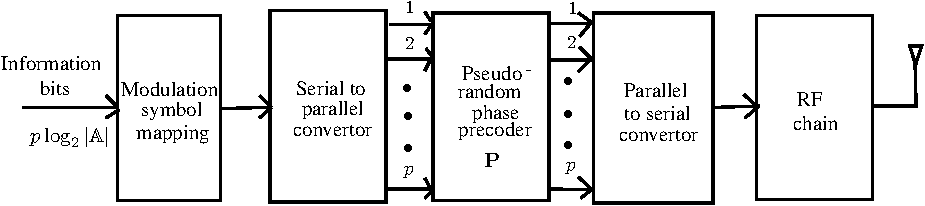
\includegraphics[scale=1]{sisoprecod.pdf}
\caption{PRPP transmitter.}
\label{prppblock}
%\end{center}
\end{figure}

\begin{eqnarray}
\vy_p&=& 
 \begin{bmatrix} 
   h_{(1)} & { 0} & \cdots & { 0} \\
   { 0}   & h_{(2)} & \cdots & { 0} \\
   \vdots & & \ddots & \vdots \\
   { 0} & { 0} & \cdots & h_{(p)}
 \end{bmatrix}\pp\mathbf s+\vn_p \nonumber\\
 &=&\md\pp\mathbf s + \vn_p=\mg\mathbf s + \vn_p,
\end{eqnarray}
where $\md=diag(h_{(1)}\, h_{(2)}\, \cdots\, h_{(p)})$, 
$\mg=\md\pp$, and $\vn_p$ is the noise vector 
$[\vn_{(1)}^T\, \vn_{(2)}^T\, \cdots\, \vn_{(p)}^T]^T$. The entries of the matrix $\mg$ are uncorrelated and 
$\lVert \md\rVert_F=\lVert \mg \rVert_F$. This creates a $p\times p$ 
virtual large-MIMO system.

The performance of PRPP transmission in a SISO system with MMSE-LAS detection algorithm [1], [2] is shown in Fig. \ref{sisoprecod}. It compares the average BER performance of the system without PRPP using ML detection against the performance of  PRPP transmission with MMSE-LAS detection. In Fig. \ref{sisoprecod}, we set the precoder size $p\in\{50,400\}$. It is interesting to note that the performance of MMSE-LAS detector approaches close to the AWGN system's performance when $p$ gets large.

\begin{figure}[htb]
\centering

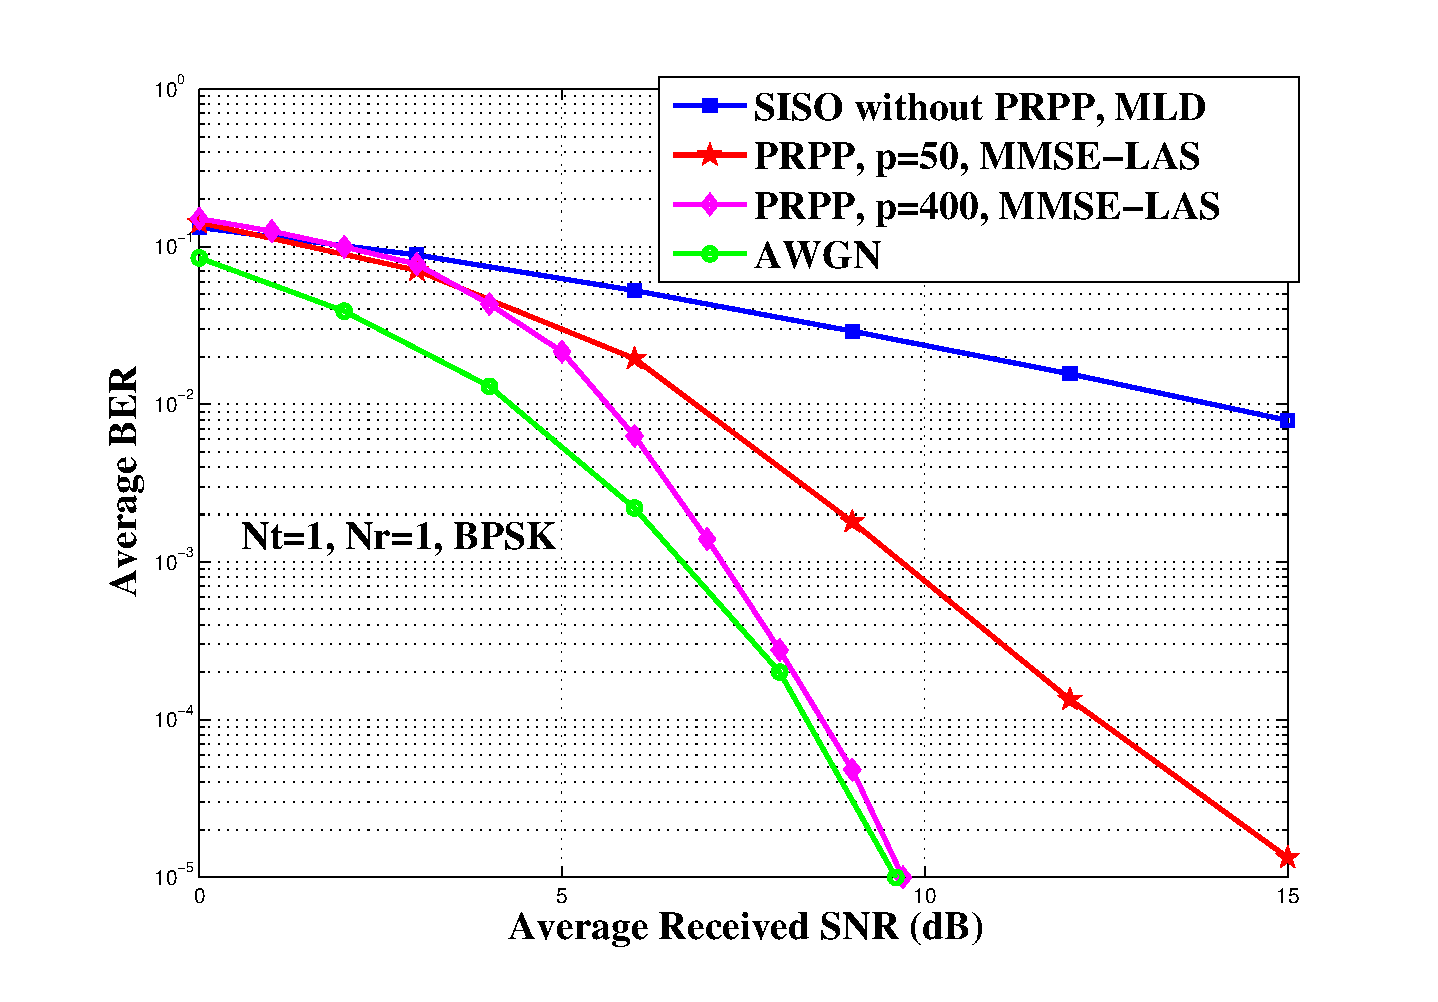
\includegraphics[totalheight=9cm,width=12cm]{rameshfig.eps}
\caption{Performance of PRPP on SISO fading channels.}
\label{sisoprecod}
%\end{center}
\end{figure}


\section{Spatial modulation}
 Spatial modulation (SM) is a transmission scheme that uses multiple transmit antennas but only one transmit RF chain [3], [4]. At each time instant, only one among all the transmit antennas will be active and the others remain silent. The index of the active transmit antenna will also convey information bits in addition to the information bits conveyed through modulation symbols (e.g., QAM). The SM transmitter is shown in Fig. \ref{smtrans}, where the transmitter has $N_t$ transmit antennas but 
only one transmit RF chain. In a given channel use, 
the transmitter selects one of its $N_t$ transmit antennas, and transmits 
a modulation symbol from the modulation alphabet ${\mathbb A}$ on the selected antenna. 
The number of bits transmitted per channel use in the modulation symbols is 
$\lfloor \log_2|{\mathbb A}| \rfloor$, and the number of bits transmitted 
per channel use by the index of the transmitting antenna is 
$\lfloor \log_2N_t \rfloor$. Therefore, a total of 
$\lfloor \log_2|{\mathbb A}| N_t \rfloor$ bits per channel use (bpcu) is 
achievable in an SM-MIMO system. For example, in a system with $N_t=2$, and
8-QAM, the system throughput is 4 bpcu. 

\begin{figure}[htb]
\centering

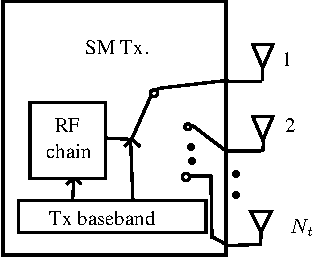
\includegraphics[scale=1]{smtransmit.pdf}
\caption{SM transmitter.}
\label{smtrans}
%\end{center}
\end{figure}

The SM alphabet set for a fixed $N_t$ and $\sa$ is given by 
\begin{eqnarray}
\sm = 
\big \{ {\bf x}_{j,l}:j=1,\cdots,N_t, \ \ l=1,\cdots,|{\mathbb A}| \big \}, \nonumber \\ 
\mbox{s.t.} \ \ {\bf x}_{j,l} = 
[0,\cdots,0,\hspace{-4mm}\underbrace{s_{l}}_{{\scriptsize{\mbox{$j$th coordinate}}}}\hspace{-3.5mm},0,\cdots,0]^T, \ \ x_l \in \mathbb{A}.  
\end{eqnarray}
For example, for $N_t=2$ and 4-QAM, ${\mathbb S}_{N_t,{\mathbb A}}$ is given by  
{\small
\begin{eqnarray}
\hspace{-4mm}
{\mathbb S}_{2,\mbox{{\tiny 4-QAM}}}  
\hspace{-3mm}&=&\hspace{-3mm}\Bigg\{ 
\begin{bmatrix} +1+j \\ 0 \end{bmatrix}, 
\begin{bmatrix} +1-j \\ 0 \end{bmatrix}, 
\begin{bmatrix} -1+j \\ 0 \end{bmatrix}, 
\begin{bmatrix} -1-j \\ 0 \end{bmatrix}, \nonumber \\ 
& & 
\begin{bmatrix} 0 \\ +1+j \end{bmatrix}, 
\begin{bmatrix} 0 \\ +1-j \end{bmatrix}, 
\begin{bmatrix} 0 \\ -1+j \end{bmatrix}, 
\begin{bmatrix} 0 \\ -1-j \end{bmatrix} 
\Bigg \}. 
\end{eqnarray}
}

\vspace{-4mm}
Let $\vx \in {\mathbb S}_{N_t,{\mathbb A}}$ denote the transmit vector.
Let $\mh \in \mathbb{C}^{N_r\times N_t}$ denote the channel gain matrix,
where $H_{i,j}$ denotes the channel gain from the $j$th transmit antenna 
to the $i$th receive antenna and these channel gains are i.i.d complex 
Gaussian random variables. The received signal at the $i$th receive 
antenna is given by
\begin{equation}
y_i = H_{i,j}x_l + n_i,
\end{equation}
where $x_l$ is the $l$th symbol in ${\mathbb A}$, transmitted by the 
$j$th antenna, and $n_i$ is the noise which is distributed as
${\mathbb C}{\mathcal N}(0,\sigma^2)$. The signal at the receiver
can be written in vector form as
\begin{eqnarray}
\vy& = & \mh\vx+\vn,
\end{eqnarray}

For this system model, the maximum-likelihood (ML) detection rule is 
given by
\begin{equation} 
\label{ml1} 
\hat{\vx}=\argmin_{\vx\in \sm} \ \|\vy-\mh\vx\|^2,  
\end{equation}



In this work, we simultaneously exploit the advantages of both SM and PRPP. We propose a novel precoded SM scheme, where both the modulation bits and the antenna index bits are precoded using 
{\em pseudo-random phases}. We refer to this system as PRPP-SM system. The proposed PRPP-SM system gives significant performance improvement over SM system  without PRPP and PRPP system without SM. Since ML detection becomes exponentially complex in large dimensions, we propose a low complexity local search based detector (LSD) suited for PRPP-SM systems with large precoder 
sizes. Our simulation results show that  the proposed PRPP-SM achieves better performance than SM system without PRPP.
\chapter{Proposed PRPP-SM system}


In this work, we propose a novel precoded SM scheme, where
both the modulation bits and the antenna index bits are precoded by
pseudo-random phases. This gives an improvement in BER performance over SM system without PRPP. This improvement increases as the precoder size increases. As ML detection becomes exponentially complex in large 
dimensions, we propose a local search detector (LSD) which scales well for large precoder 
sizes. 

\section{System model}
The proposed PRPP-SM transmitter is shown in Fig. \ref{smprecod}.
First, $p$ modulated symbols are 
accumulated  to form the symbol vector $\vx_s \in \sa^p$, where $\mathbb A$ denotes the modulation alphabet. Let the matrix $\ma$ denote the antenna activation pattern, 
such that $\ma\vx_s \in \sm^p$, where $\sm$ denotes the SM alphabet set for a fixed $N_t$ and $\mathbb A$ is given by \begin{eqnarray}
\sm = 
\big \{ {\bf x}_{j,l}:j=1,\cdots,N_t, \ \ l=1,\cdots,|{\mathbb A}| \big \}, \nonumber \\ 
\mbox{s.t.} \ \ {\bf x}_{j,l} = 
[0,\cdots,0,\hspace{-4mm}\underbrace{s_{l}}_{{\scriptsize{\mbox{$j$th coordinate}}}}\hspace{-3.5mm},0,\cdots,0]^T, \ \ x_l \in \mathbb{A}.  
\end{eqnarray} The matrix $\ma$ consists of $p$ 
submatrices such that $\ma=[\ma_{(1)}^T \, \ma_{(2)}^T \, \cdots \, \ma_{(p)}^T]^T$, where $\mathbf A_{(i)}$ is the $i$th submatrix. The submatrix $\ma_{(i)}$ indicates the antenna activated in the
$i$th channel use. $\ma_{(i)}$ is a $N_t\times p$ matrix constructed as 
\begin{eqnarray}
\ma_{(i)}=[{\bf 0}_{(1)} \, \cdots \, {\bf 0}_{(i-1)} \, {\bf a}_{(i)} \, {\bf 0}_{(i+1)} \, \cdots \, {\bf 0}_{(p)}],
\end{eqnarray} 
where ${\bf 0}_{(k)}$ is a $N_t\times 1$ vector of zeroes, and 
${\bf a}_{(i)}$ is a $N_t\times 1$ vector constructed as
$[0 \, \cdots \, 0 \, \hspace{-2mm}\underbrace{1}_{\mbox{\tiny{$j_i$th coordinate}}} \hspace{-2mm} 0 \, \cdots \, 0]^T$, and $j_i$ is the index of the active antenna
during the $i$th channel use.

For example, in a system with $N_t=2$ and $p=3$, to activate antennas
1, 2 and 1 in three consecutive channel uses, respectively, the matrix 
$\ma$ is given by

\begin{figure}[t]
\centering

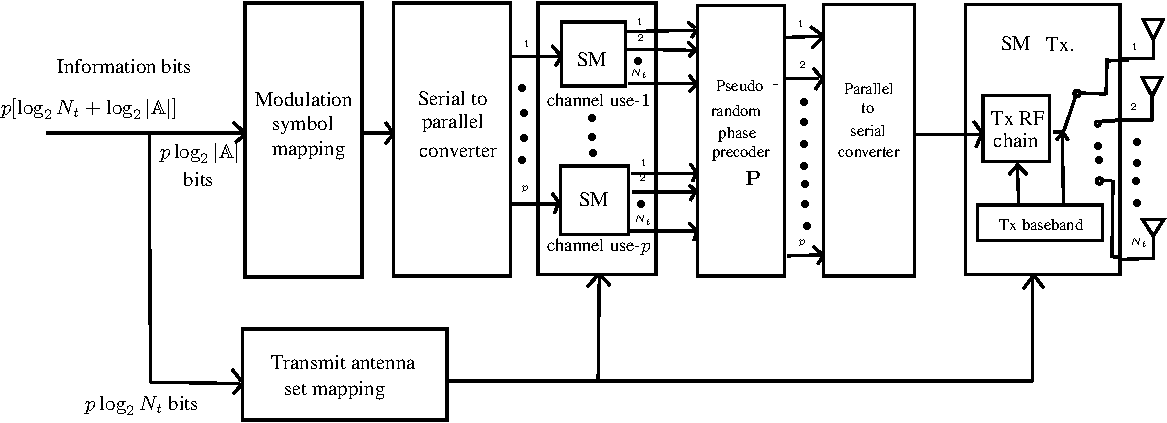
\includegraphics[scale=0.8]{rppsm.pdf}
\caption{Proposed PRPP-SM transmitter.}
\label{smprecod}
%\end{center}
\end{figure}

\begin{eqnarray}
\begin{bmatrix}
\ma_{(1)}\\
\ma_{(2)}\\
\ma_{(3)}
\end{bmatrix}&=&
 \begin{bmatrix}
1 & 0 & 0\\
0 & 0 & 0\\ \hdashline
0 & 0 & 0\\
0 & 1 & 0\\ \hdashline
0 & 0 & 1\\
0 & 0 & 0
 \end{bmatrix}
\end{eqnarray}

The matrix $\ma$ gives the support of the spatially modulated transmit
vector. The vector $\ma\vx_s \in \sm^p$ is precoded using a $p \times pN_t$ matrix $\pp$ to get $\pp\ma\vx_s$. 
The $(r,c)$th entry of the matrix $\pp$ is
$\frac{1}{\sqrt{p}}}e^{j\theta_{r,c}}$, where the phases 
$\theta_{r,c}$s are generated using a pseudo-random sequence generator. The seed of this generator is pre-shared among the transmitter and 
receiver. The output of the precoder is transmitted on the selected antenna in each channel use.
The signal received at the receiver after $p$ channel uses is given by
\begin{eqnarray}
\vy_p&=& 
 \begin{bmatrix} 
   \mh_{(1)} & {\bf 0} & \cdots & {\bf 0} \\
   {\bf 0}   & \mh_{(2)} & \cdots & {\bf 0} \\
   \vdots & & \ddots & \vdots \\
   {\bf 0} & {\bf 0} & \cdots & \mh_{(p)}
 \end{bmatrix}\ma\pp\ms\vx_s+\vn_p \nonumber\\
 &=&\md\ma\pp\ma\vx_s + \vn_p,
\end{eqnarray}
where $\md=diag(\mh_{(1)}\, \mh_{(2)}\, \cdots\, \mh_{(p)})$,  
 and $\vn_p$ is the noise vector 
$[\vn_{(1)}^T\, \vn_{(2)}^T\, \cdots\, \vn_{(p)}^T]^T$. For this system model, the ML detection rule is 
given by
\begin{equation} 
\label{ml3} 
\{\hat{\vx}_s,\hat{\ma}\}=\argmin_{\vx_s\in \sa^p, \forall \ma} \ \|\vy_p-\md\ma\pp\ma\vx_s\|^2,  
\end{equation}

The index of the non-zero row in each submatrix of  $\hat{\mathbf A}$ and values of $\hat{\mathbf x}_s$ are demapped to obtain the information bits.


\section{Proposed detection algorithm}

From (\ref{ml3}), it can be seen that the ML detection of the transmitted 
bits in a precoded SM-MIMO system is exponential in complexity, i.e.,
$O(|\sa|n_t)^p)$. We propose a local search based detector (LSD)
that achieves near-ML detection at large $p$ with a low computational 
complexity. The local search detector obtains a local minima in terms of
the least ML cost among a local neighborhood. The neighborhood is defined as follows. The set of neighbors of a given
pair of $\{\ma, \vx_s\}$, denoted by ${\mathcal N}(\ma, \vx_s)$, is defined as the 
set of all pairs $\{\ma', \vx_s'\}$ that satisfies one of the following 
three conditions:
\begin{enumerate}
\item
$\vx_s=\vx_s'$ and $\ma_{(i)}\neq\ma_{(i)}'$ for exactly a single index
$i$
\item 
$\ma=\ma'$ and $\vx_s$ differs from $\vx_s'$ in exactly one entry
\item
$\ma_{(i)}\neq\ma_{(i)}'$ for exactly a single index $i$, and for that 
index $i$, $x_s(i)\neq x'_s(i)$.
\end{enumerate}

For example, consider $N_t$=2, $p$=2, and  $\sa=\{\pm1\}$.  Then, we have
 


\vspace{0.5cm}
${\small
{\cal N}\left(\begin{bmatrix} 1&0 \\ 0&0 \\\hdashline 0&0 \\0&1\end{bmatrix},\begin{bmatrix} +1 \\ -1\end{bmatrix}\right)
\hspace{-1mm}=\hspace{-1mm}\left\{\begin{matrix}\vspace{0.5cm}
\{\begin{bmatrix} 1&0 \\ 0&0 \\\hdashline 0&1 \\0&0\end{bmatrix},\begin{bmatrix} +1 \\ -1\end{bmatrix}\},
\{\begin{bmatrix} 1&0 \\ 0&0 \\\hdashline 0&1 \\0&0\end{bmatrix},\begin{bmatrix} +1 \\ +1\end{bmatrix}\},
\{\begin{bmatrix} 1&0 \\ 0&0 \\\hdashline 0&1 \\0&0\end{bmatrix},\begin{bmatrix} -1 \\ -1\end{bmatrix}\},
\{\begin{bmatrix} 1&0 \\ 0&0 \\\hdashline 0&0 \\0&1\end{bmatrix},\begin{bmatrix} -1 \\ -1\end{bmatrix}\}\\

\vspace{0.5cm}


 \{\begin{bmatrix} 1&0 \\ 0&0 \\\hdashline 0&0 \\0&1\end{bmatrix},\begin{bmatrix} +1 \\ +1\end{bmatrix}\},
\{\begin{bmatrix} 0&0 \\ 1&0 \\\hdashline 0&0 \\0&1\end{bmatrix},\begin{bmatrix} +1 \\ -1\end{bmatrix}\},
\{\begin{bmatrix} 0&0 \\ 1&0 \\\hdashline 0&0 \\0&1\end{bmatrix},\begin{bmatrix} +1 \\ +1\end{bmatrix}\},
\{\begin{bmatrix} 0&0 \\ 1&0 \\\hdashline 0&0 \\0&1\end{bmatrix},\begin{bmatrix} -1 \\ -1\end{bmatrix}\}\end{matrix}
\right\}.
}$

The proposed LSD algorithm starts with an intial solution $\{\ma^{(0)}, \vx_s^{(0)}\}$, 
which is also the current solution. Using the defined neighborhood, the 
algorithm considers all the neighbors of $\{\ma^{(0)}, \vx_s^{(0)}\}$ and searches 
for the neighbor with the least ML cost which also has a lower ML cost 
than the current solution. If such a neighbor is found, then this neighbor 
is designated as the current solution. This marks the completion of one 
iteration of LSD. The iterations are repeated till a local minima is 
reached (i.e., there is no neighbor better than the current solution).  
The solution corresponding to the local minima is declared as the final 
output $\{\hat{\ma}, \hat{\vx}_s\}$. This algorithm is listed in 
{\bf Algorithm \ref{algo}}.

\begin{algorithm}[t]      
\caption{Listing of the proposed LSD}
   \begin{algorithmic} [1] 
      \STATE $\mathbf{Input: y, H}$,$\mathbf P$      
      \STATE Intial solution : $\{\ma^{(0)}, \vx_s^{(0)}\}$,  $\{\hat{\ma}, \hat{\vx}_s\}=\{\ma^{(0)}, \vx_s^{(0)}\}$
      \STATE Compute ${\cal N}(\hat{\ma}, \hat{\vx}_s)$
      \STATE $\{\ma^c, \vx_s^c\}$ = $\argmin\limits_{\{\mb,\vz\}\in{\cal N}(\hat{\ma}, \hat{\vx}_s)} \, \|\vy_p-\md\mb\pp\mb\vz\|^2$
	\IF{ $\|\vy_p-\md\ma^c\pp\ma^c\vx_s^c\|^2 < \|\vy_p-\md\hat{\ma}\pp\hat{\ma}\hat{\vx}_s\|^2 $}
	\STATE  $\{\hat{\ma}, \hat{\vx}_s\}=\{\ma^c, \vx_s^c\}$
	\STATE  Go to step 3
	\ENDIF 
      \STATE $\mathbf{Output}$ : $ \{\mathbf {\hat{A}},\mathbf {\hat{s}}\}$
\vspace{3mm}
\end{algorithmic}
\label{algo}
\end{algorithm} 

{\em Computing the intial solution}: We use MMSE for estimating the support and to 
obtain the initial solution to the LSD algorithm.  The MMSE
estimate is a $pN_t\times 1$ vector given by
$\vv=(\md^H\md+\sigma^2\mi)^{-1}\md^H\vy_p$. The vector $\vv$
consists of $p$ subvectors of size $N_t\times 1$,
$\vv=[\vv_{(1)}^T \,\vv_{(2)}^T \, \cdots \, \vv_{(p)}^T]^T$.
The indices of the elements with the largest amplitude in each
$\vv_{(i)}$ gives the initial solution for $\ma^{(0)}$. The  MMSE estimate of  $\vx_s ^{(0)}$ is given by a $p\times 1$ vector given by
$\vz=(\mg^H\mg+\sigma^2\mi)^{-1}\mg^H\vy_p$, where $\mathbf G=\mathbf H\mathbf \ma^{(0)}\mathbf P\mathbf \ma^{(0)} $. The hard estimate of $\vx_s^{(0)} $  is obtained by mapping each coordinate of $\vz$ to nearest symbol in the alphabet in terms of Euclidean distance.

\section{Simulation results}

We present the simulation results on the performance of the proposed PRPP-SM system with ML detection and MMSE-LSD. In all our simulations,  the channel is assumed to undergo temporally uncorrelated Rayleigh fading and independent between channel uses. 

Figure \ref{smml} compares the performance of PRPP-SM against the performance of SM without PRPP at a spectral efficiency of 3 bpcu using ML detection. Here, $N_t=4, N_r=1$ and BPSK modulation is used with precoder size  $ p \in\{2,4,5\}$. It is interesting to note that the performance of PRPP-SM is better than SM without PRPP by about 9 dB at $p=5$ and $10^{-2}$ BER. The performance of PRPP-SM gets even  better as $p$ increases.

Figure \ref{sisoml} compares the performance of PRPP-SM against the performance of PRPP without SM (i.e. $N_t=1$) at a spectral efficiency 3 bpcu using ML detection. Here, the PRPP-SM system has $N_t=4, N_r=1$, BPSK modulation, and PRPP system without SM  has $N_t=1, N_r=1$, 8-QAM  with precoder size  $ p \in\{2,4,5\}$. It is noted that the performance of PRPP-SM is better than the PRPP without SM by about 4 dB at $p=5$ and $10^{-2}$ BER. 

Figure \ref{smmmselas} compares the performance of PRPP-SM using MMSE-LSD detection against the performance of SM without PRPP using MLD at a spectral efficiency of 2 bpcu. Here PRPP-SM with $N_t=2, N_r=4$, and BPSK modulation is used with precoder size  $ p \in\{10,20,70\}$. It is seen that for smaller precoder sizes, PRPP-SM  performs poorer than SM without PRPP. But as the  precoder size increases, PRPP-SM performs better than SM without PRPP. At $10^{-5}$ BER, PRPP-SM with $p=70$ using MMSE-LSD detection is 1 dB  better than SM without PRPP using ML detection. This performance advantage in favor of PRPP-SM is expected to be even better for large values of $p$.

Figure \ref{sisolas} compares the performance of PRPP-SM using MMSE-LSD detection against the performance of PRPP without SM using MMSE-LAS detection, at a spectral efficiency 3 bpcu. For PRPP-SM we have used $N_t=4, N_r=8$, BPSK modulation. For PRPP without SM  we have used $N_t=1, N_r=8,$ 8-QAM.  The precoder size  $ p \in\{10,20,70\}$ in both systems. The spectral efficiency in both systems is 3 bpcu. It is observed that the performance of  PRPP-SM system is better than the PRPP system without SM by about 10 dB at $p$ = 70 and $10^{-2}$ BER. 






\begin{figure}[htb]
\centering

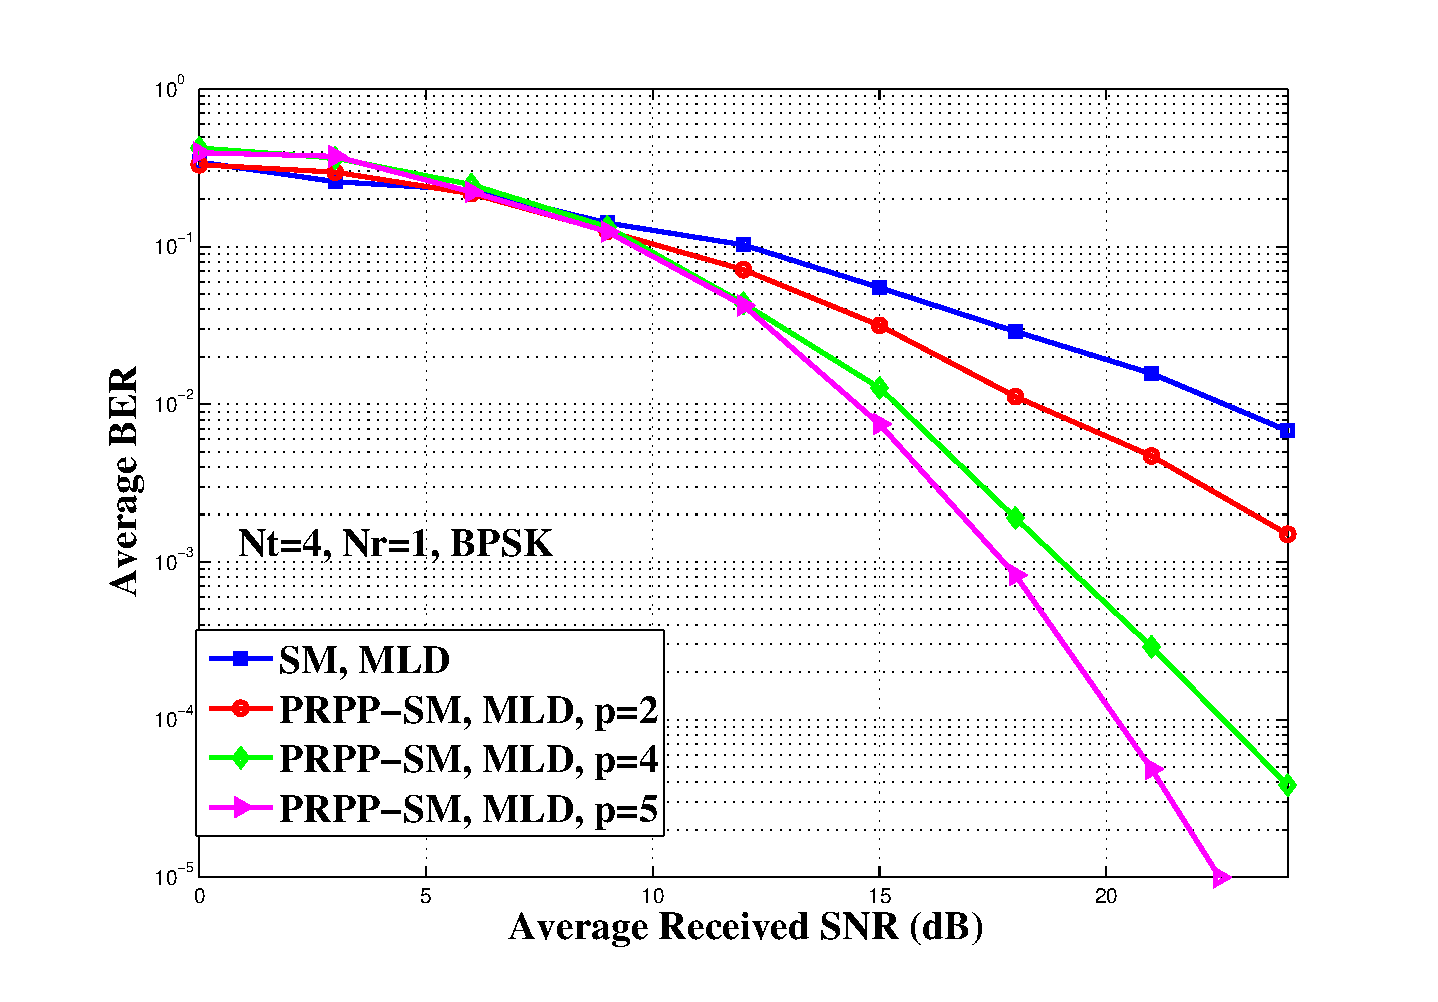
\includegraphics[totalheight=9cm,width=12cm]{prpp_sm_vs_withoutsm_ml.eps}
\caption{Performance comparison between PRPP-SM system $(N_t=4, N_r=1$, BPSK) with ML detection  and SM system without PRPP with ML detection. 3 bpcu.}
\label{smml}
%\end{center}
\end{figure}

\begin{figure}[htb]
\centering

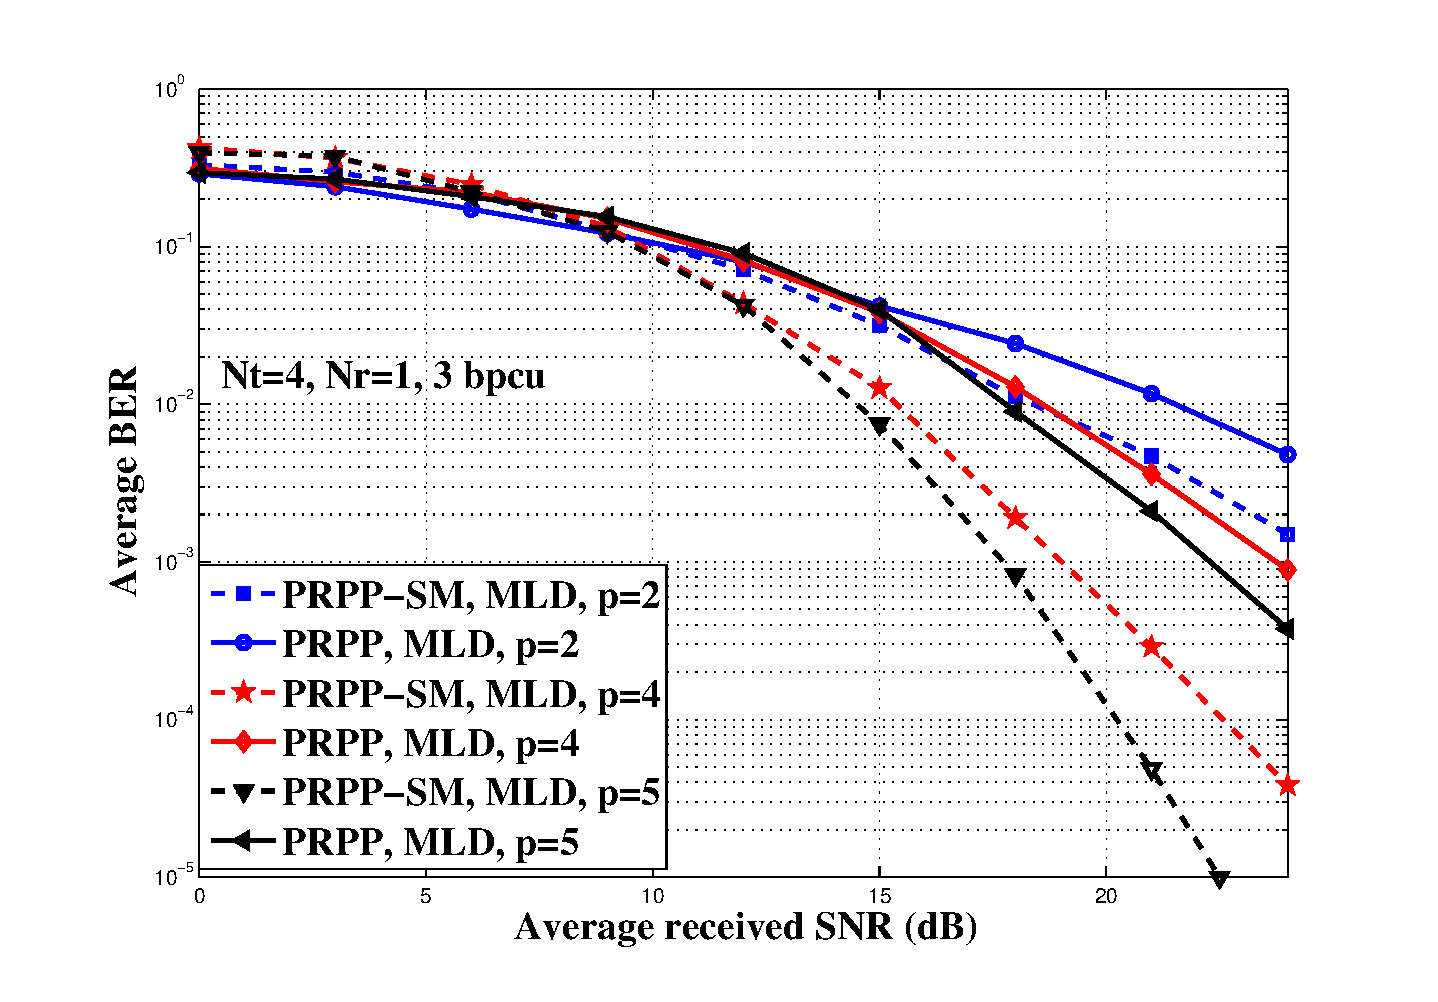
\includegraphics[totalheight=9cm,width=12cm]{prppsiso_vs_sm_ml.eps}
\caption{Performance comparison between PRPP-SM system $(N_t=4, N_r=1$, BPSK) with ML detection  and  PRPP without SM $(N_t=1, N_r=1$, 8-QAM) with ML detection. 3 bpcu.}
\label{sisoml}
%\end{center}
\end{figure}

\begin{figure}[htb]
\centering

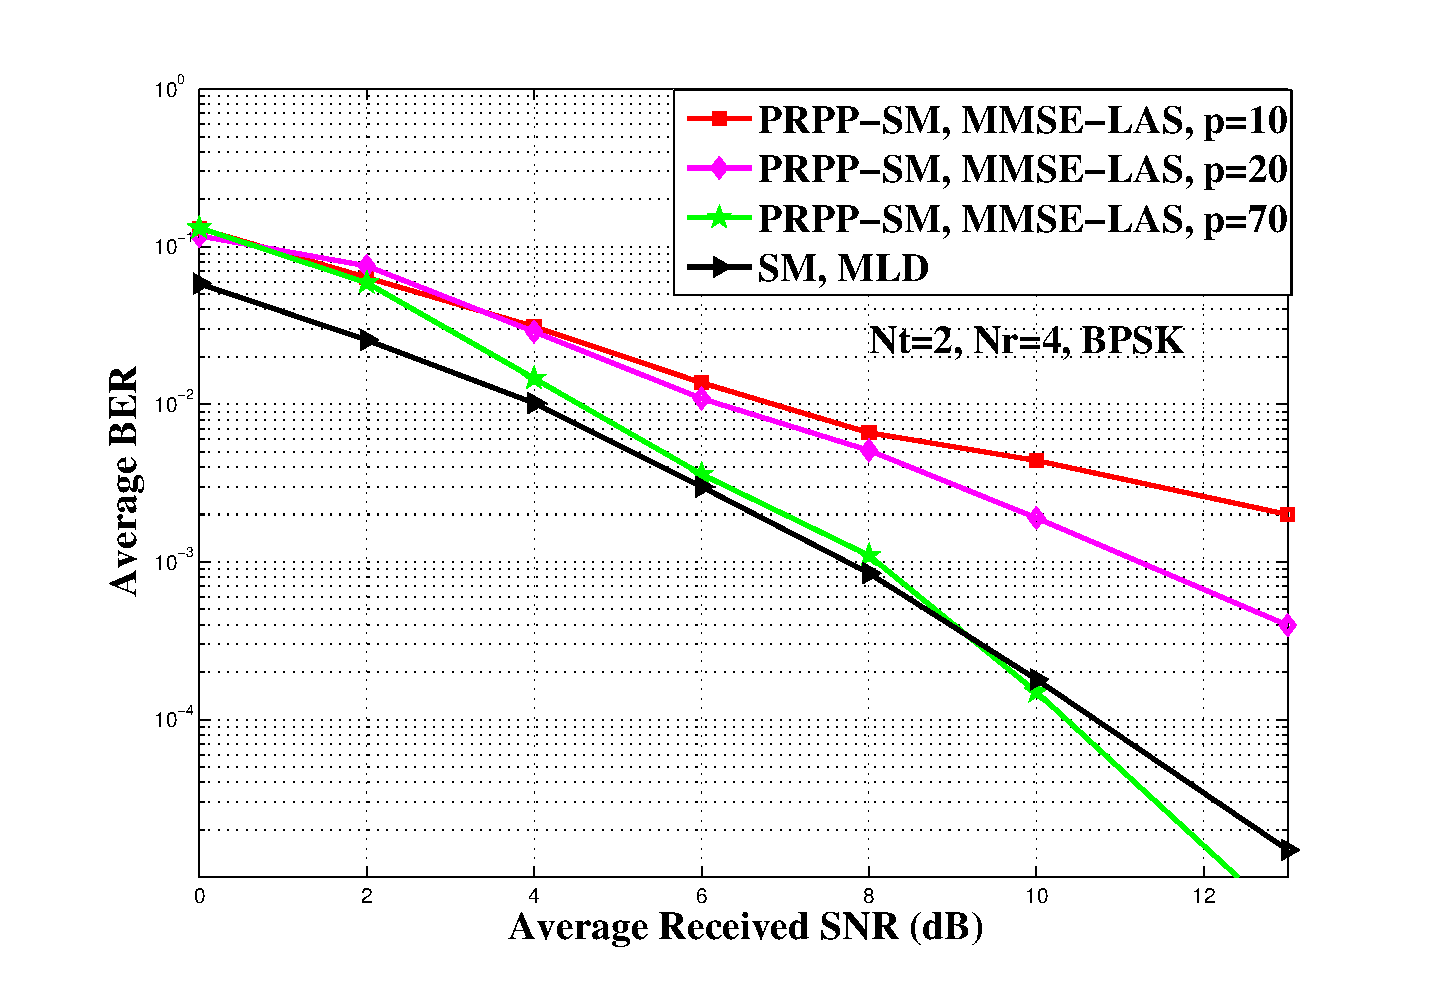
\includegraphics[totalheight=9cm,width=12cm]{prpp_sm_vs_withoutsm_mmse_las.eps}
\caption{Performance comparison between PRPP-SM $(N_t=2, N_r=4,$ BPSK) with LSD detection  and SM system without PRPP using ML detection. 2 bpcu.}
\label{smmmselas}
%\end{center}
\end{figure}
\begin{figure}[htb]
\centering

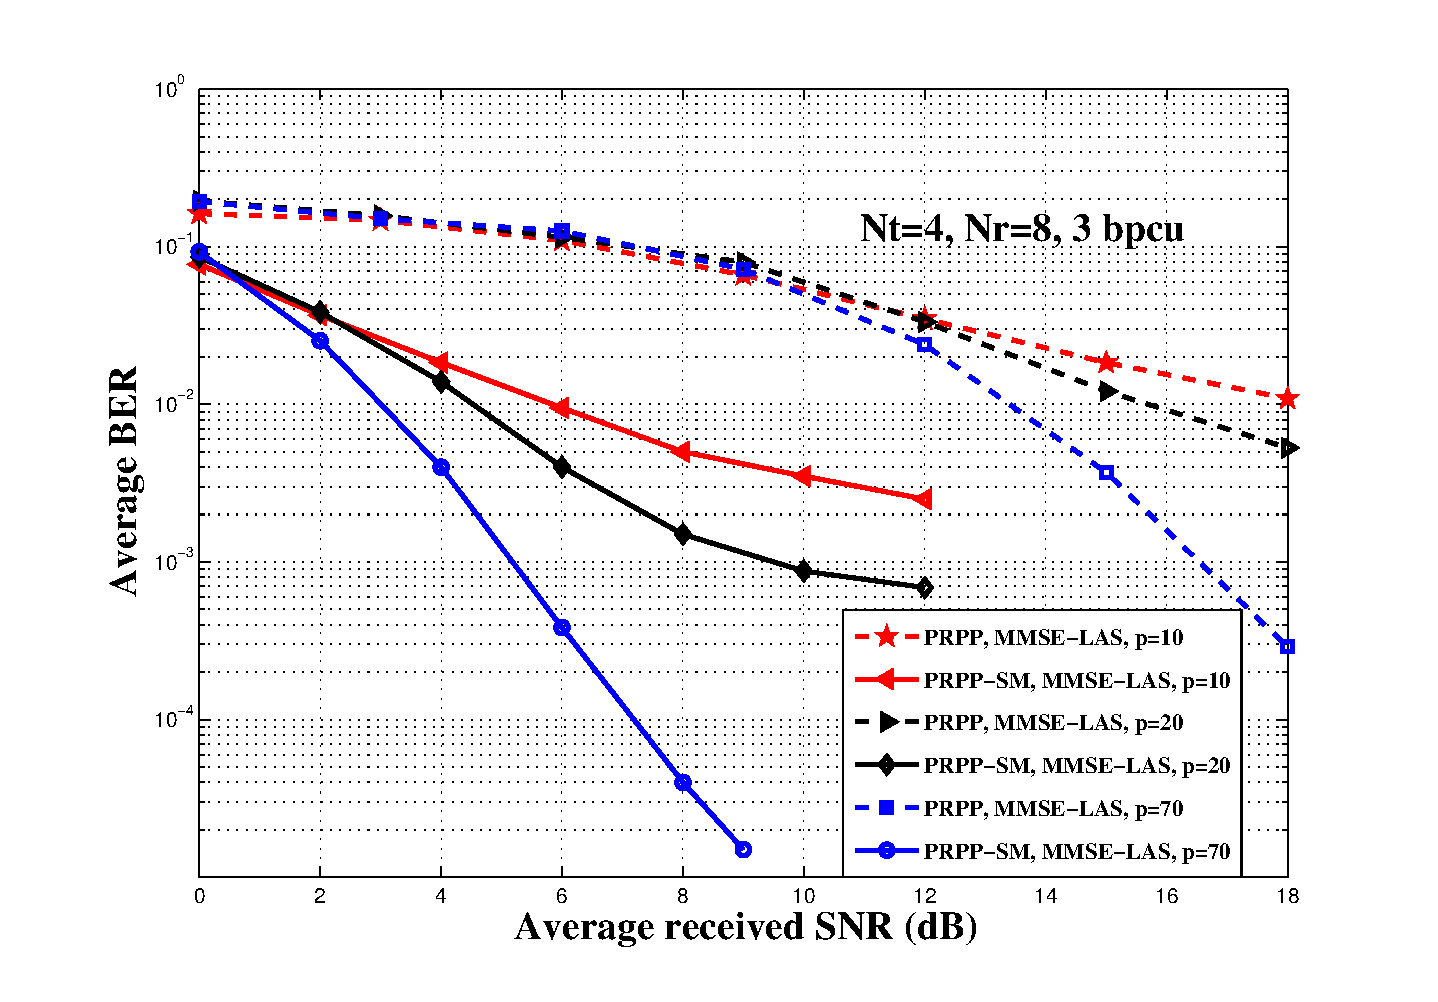
\includegraphics[totalheight=9cm,width=12cm]{prpp_sm_las.eps}
\caption{Performance comparison between PRPP-SM system $(N_t=4, N_r=8$, BPSK) with LSD detection  and PRPP without SM $(N_t=1,N_r=8$, 8-QAM) with LSD detection. 3 bpcu.}
\label{sisolas}
%\end{center}
\end{figure}


   
   \chapter{Conclusions and future work}
   
   We proposed a novel pseudo-random phase precoder based spatial modulation (PRPP-SM)  schemefor uncoded transmissions over fading channels. We assumed channel fades are independent and identically distributed across channel uses. With $N_t=4,N_r=1$, BPSK modulation, and ML detection, we demonstrated that the proposed PRPP-SM system achieves better performance than SM system without precoding and PRPP system without SM. We also proposed low complexity local search algorithm for detection in PRPP-SM systems  with large precoder sizes.
   With $N_t=4, N_r=1$, BPSK modulation, $5\times20$ precoder matrix and ML detection, we demonstrated that the proposed PRPP-SM system achieves better performance than the SM system without PRPP with ML detection by about 9 dB at $10^{-2}$ BER. The proposed system achieves increased diversity as the precoder size increases. In future, we will investigate the effect of time correlation on the performance of the PRPP-SM system.
   
  

 \begin{thebibliography}{99}
\vspace{0mm}

\bibitem{ic1}
R. Annavajjala and P. V. Orlik, ``Achieving near exponential diversity on uncoded low-dimensional MIMO, multi-user and multi-carrier systems without transmitter CSI, '' \textit{ Proc. ITA'2011}, Jan. 2011.
\bibitem{ic2} 
 K. V. Vardhan, S. K. Mohammed, A. Chockalingam, and B. S. Rajan,
``A low-complexity detector for large MIMO systems and multicarrier
CDMA systems,``\textit{ IEEE Journal on Selected Areas in Comm.}, vol. 26,
no. 3, pp. 473-485, Apr. 2008.

\bibitem{ic3} 
 R. Mesleh, H. Hass, S. Sinaovic, C. W. Ahn, ``Spatial modulation,''\textit{IEEE Trans.Veh.Tech.}, vol. 57, no. 4, pp. 2228-2241, Jul. 2008.
 
\bibitem{ic4}
 M. Di Renzo, H. Haas, A. Ghrayeb, S. Sugiura, and L. Hanzo, ``Spatial
modulation for generalized MIMO: challenges, opportunities and 
implementation,'' {\em Proceedings of the IEEE}, vol. 102, no. 1, pp. 53-55, Jan. 2014. 




\end{thebibliography}      
      



\end{document}